\chapter{Using \agentj}
\label{jnipai}

Using \agentj, a Java NS2 agent can be attached to an NS2 node and
can be used to integrate any Java application. This chapter gives an 
overview of the interaction between the 
TCL scripts, the C++ NS2 agents and Java objects, which can be accessed from each
NS2 node.  The various code snippets are taken from the \agentj~
source tree and pointers are referenced relative to the
installation directory, when provided. 


\begin{figure}
\centering
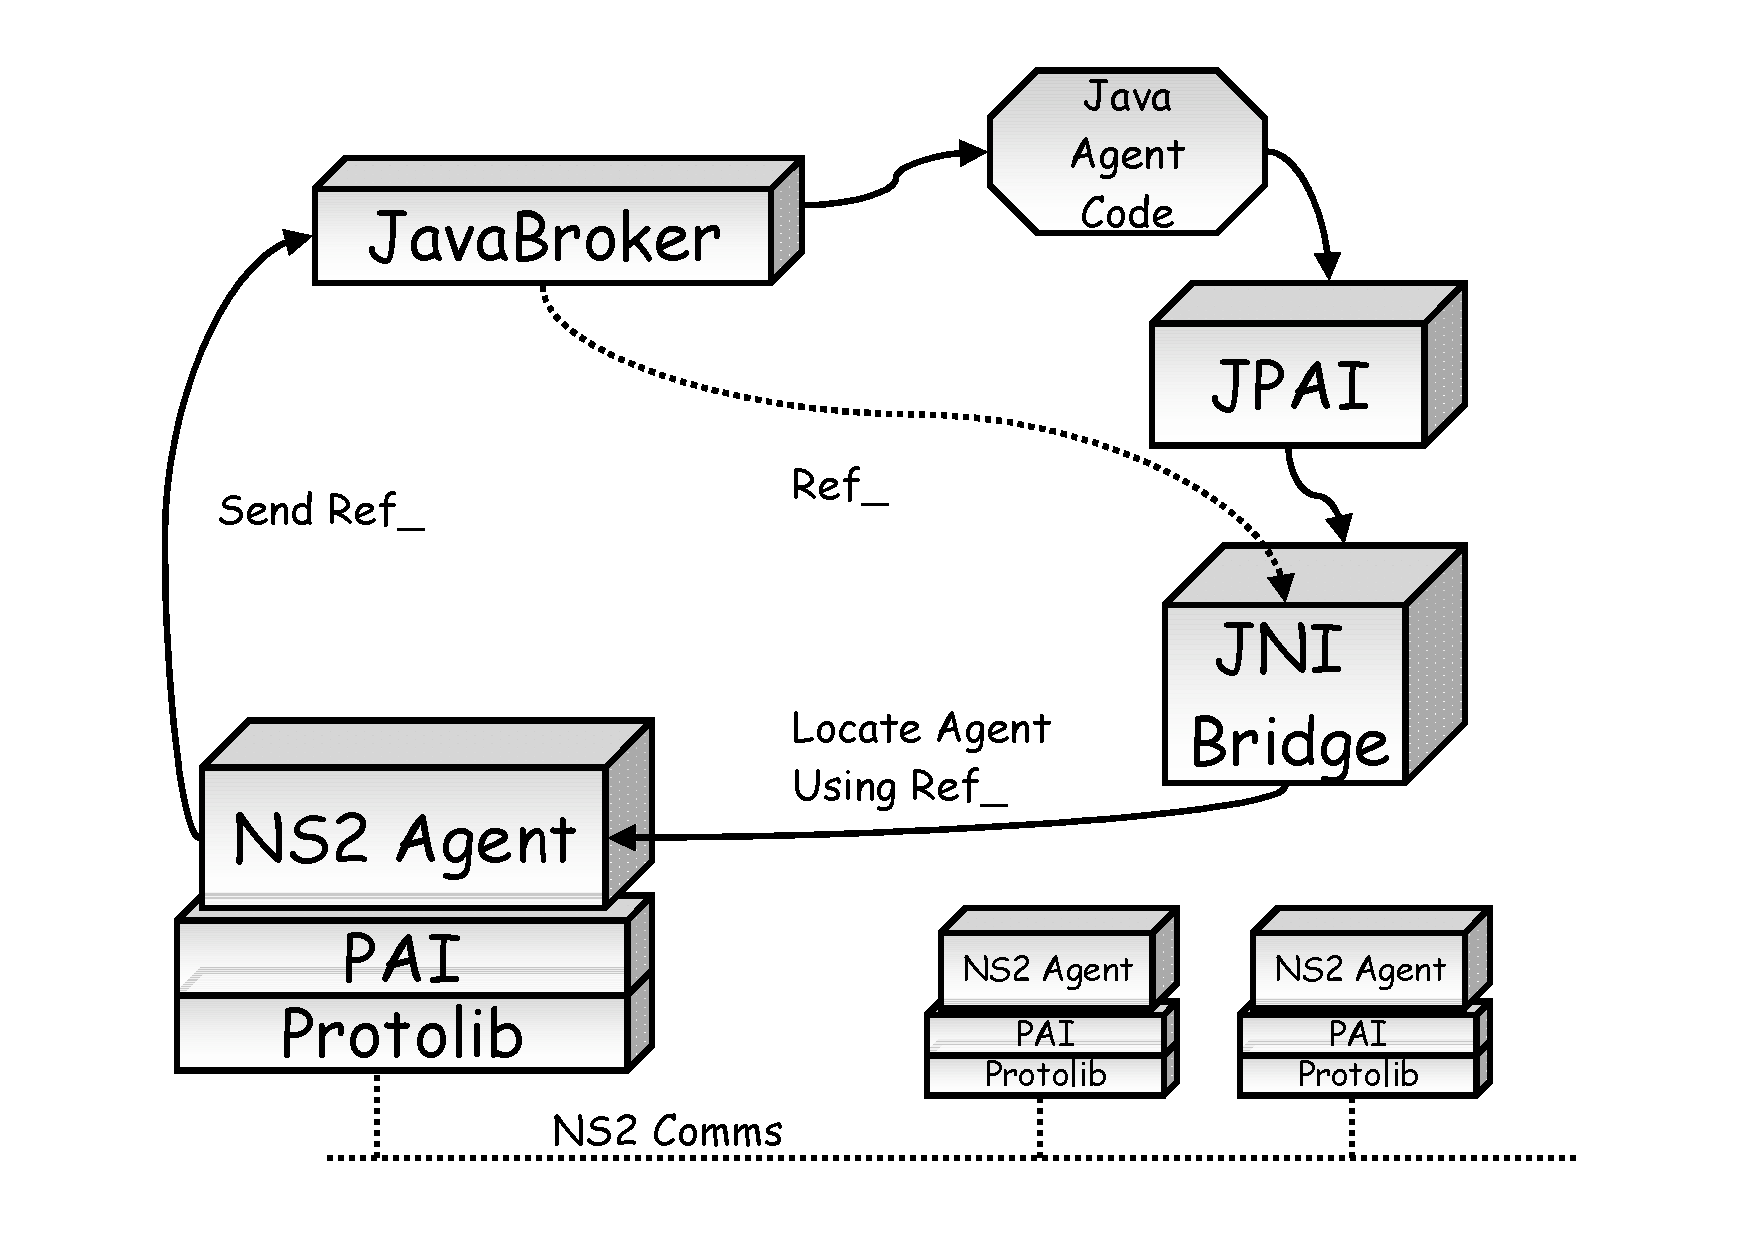
\includegraphics[scale=0.4]{images/agentjJNIOverview}
\caption{An overview PAI is accessed from within a Java node for an NS2 agent} 
\label{jnipai:fig:overview}
\end{figure}

Figure \ref{jnipai:fig:overview} shows an overview of the 
interaction between the C++ agents, the \emph{JavaBroker}
and the Java PAI bridge that enables this to be interfaced with
the C++ PAI library. As discussed briefly in the previous
chapter, the C++  \emph{JavaAgent} passes the pointer to the C++
agent to the  \emph{JavaBroker} when it requests to create and
attach a Java agent to the NS2 node.  

The  \emph{JavaBroker}
class uses this pointer to store the created Java object in
a hashtable for lookup but also pass this references across to
the JNI interface, when a Java object requires the use of 
the PAI interface. This enables the JNI interface to locate the
node that created the Java object and therefore whom is
indirectly issuing the commands, which ensures that 
the data being sent through the sockets is sent from 
the correct node.  The PAI interface sends these commands
to the Protolib library, which in turn, uses the Protolib NS2 UDP
implementation to send the data between the NS2 nodes.


\section{Invoking Java Agents from NS2 Agents}
\label{jni:invoke}

Figure \ref{jni:fig:javaVM} shows interaction between an agent and 
its associated Java class.  The programmer who wishes to use this
Java functionality within their NS2 simulations only needs to be 
concerned within their NS2 TCL script and their Java class that 
implements the behaviour. The relationship between an Ns2 agent 
and its Java class is very similar to the relationship between an NS2
TCL script and its associated C++ class (i.e. an NS2 agent) which 
implements the same kind of interaction through sending text
commands between the two. The Java interface
employs the same mechanism to bridge these different 
programming languages. The C++ agent (JavaAgent) simply acts
as a go-between and passes that commands across to the
appropriate Java object. 

\begin{figure}
\centering
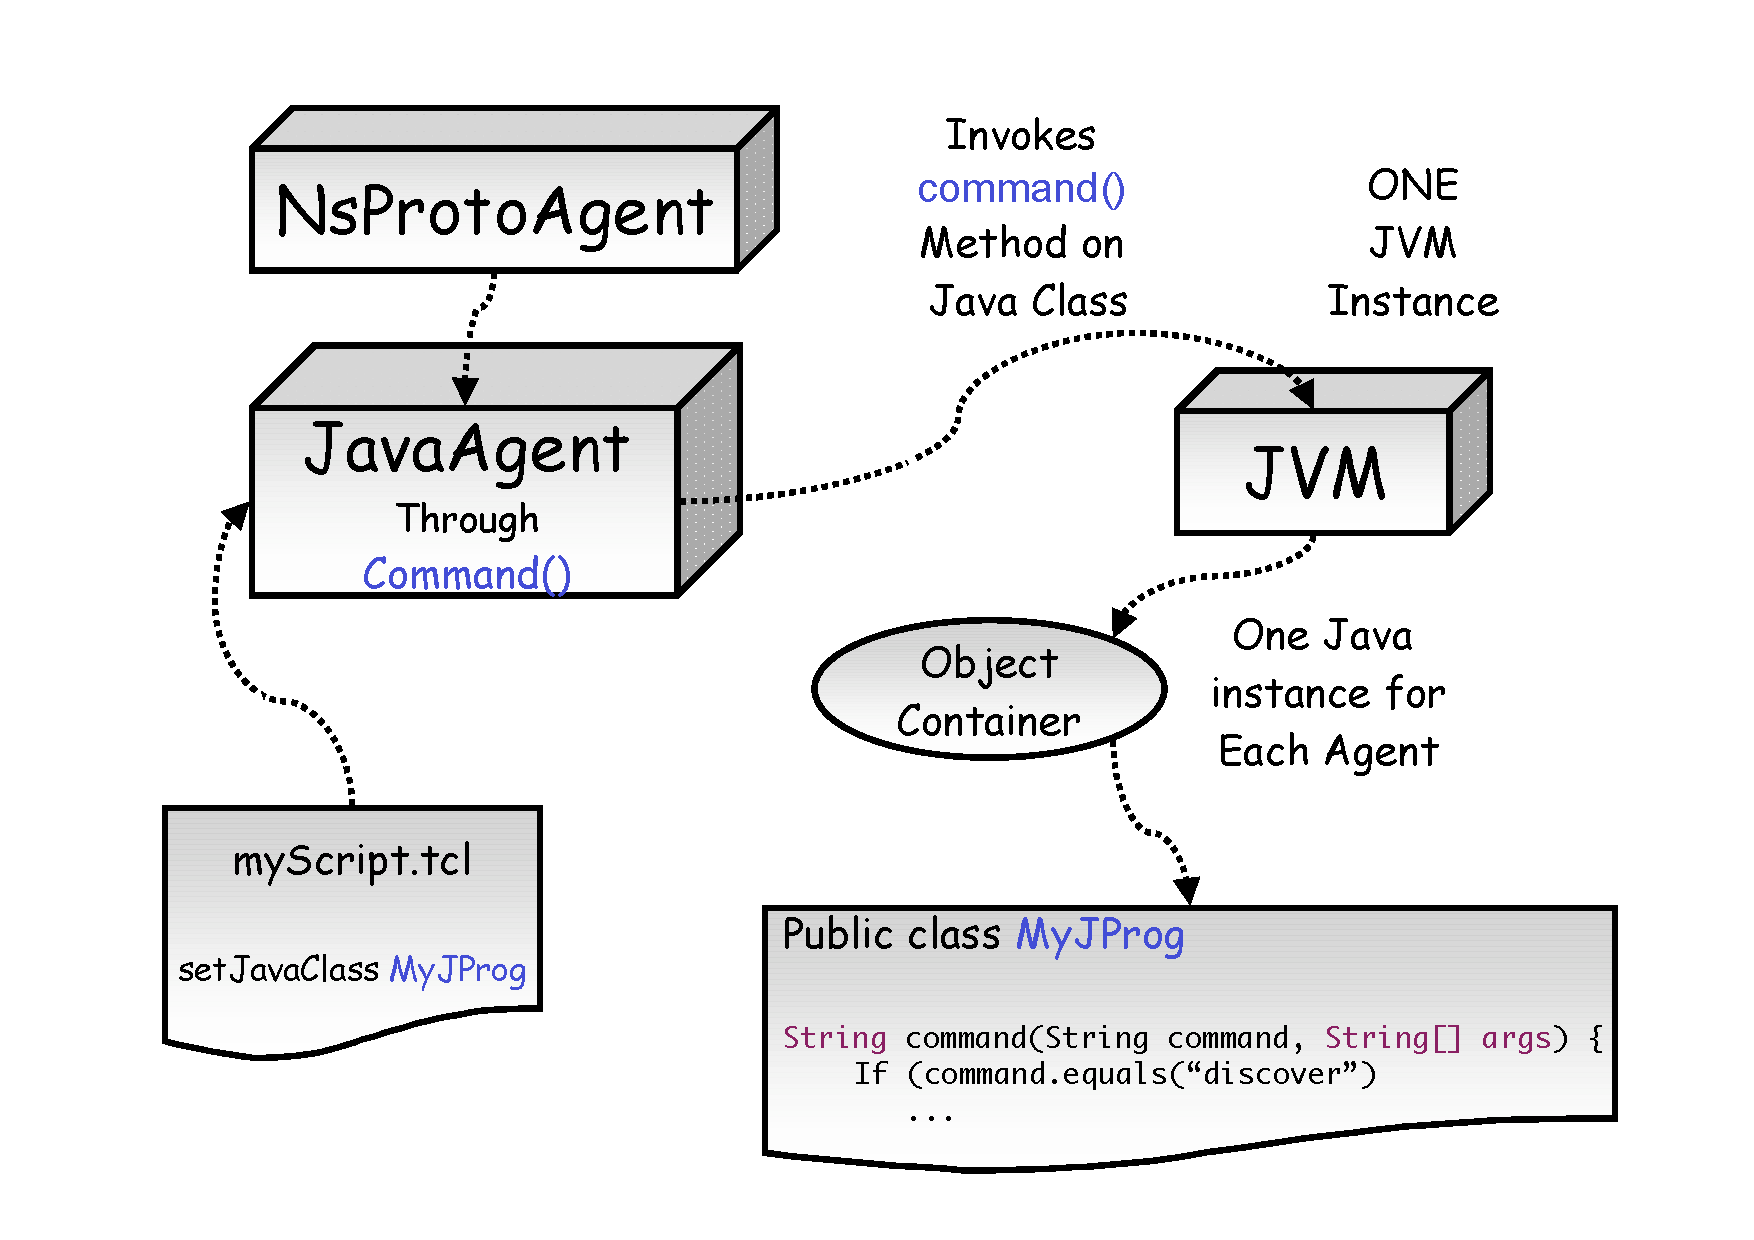
\includegraphics[scale=0.4]{images/agentuserJVM}
\caption{The interface to a Java program for an agent employs 
a similar interface to that of NS2 when communicating between 
the TCL scripts and the C++ classes. } 
\label{jni:fig:javaVM}
\end{figure}

Therefore, the interface between the NS2 \emph{JavaAgent} 
and the chosen Java Class it will interact with, uses the same 
command-style interface as the TCL-C++ interface for invoking 
functionality on NS2 agents. This command-style interaction 
satisfies some essential constraints:

\begin{itemize}
\item \textbf{Flexibility:} it will keep the flexibility of being able to use NS2 agents in any way programmer sees fit - the Java extensions are optional and any agent extending
the \emph{JavaAgent} can choose to use this functionality. However, the core
C++ agent code can be programmed to incorporate and other functionality 
needed beyond the scope of Java. 
\item  \textbf{Simplicity:} the scalability issues and framework for interacting with
the Java objects can easily be hidden behind the container C++ and Java classes 
- the programmer does not need to be aware of their presence.
\item  \textbf{Familiarity:} this mechanism allows communication between the 
NS2 agent and any attached Java class through the same familiar interface as NS2 programmers interface between the TCL scripts and C++ agents now.
\end{itemize}

\begin{figure}
\centering
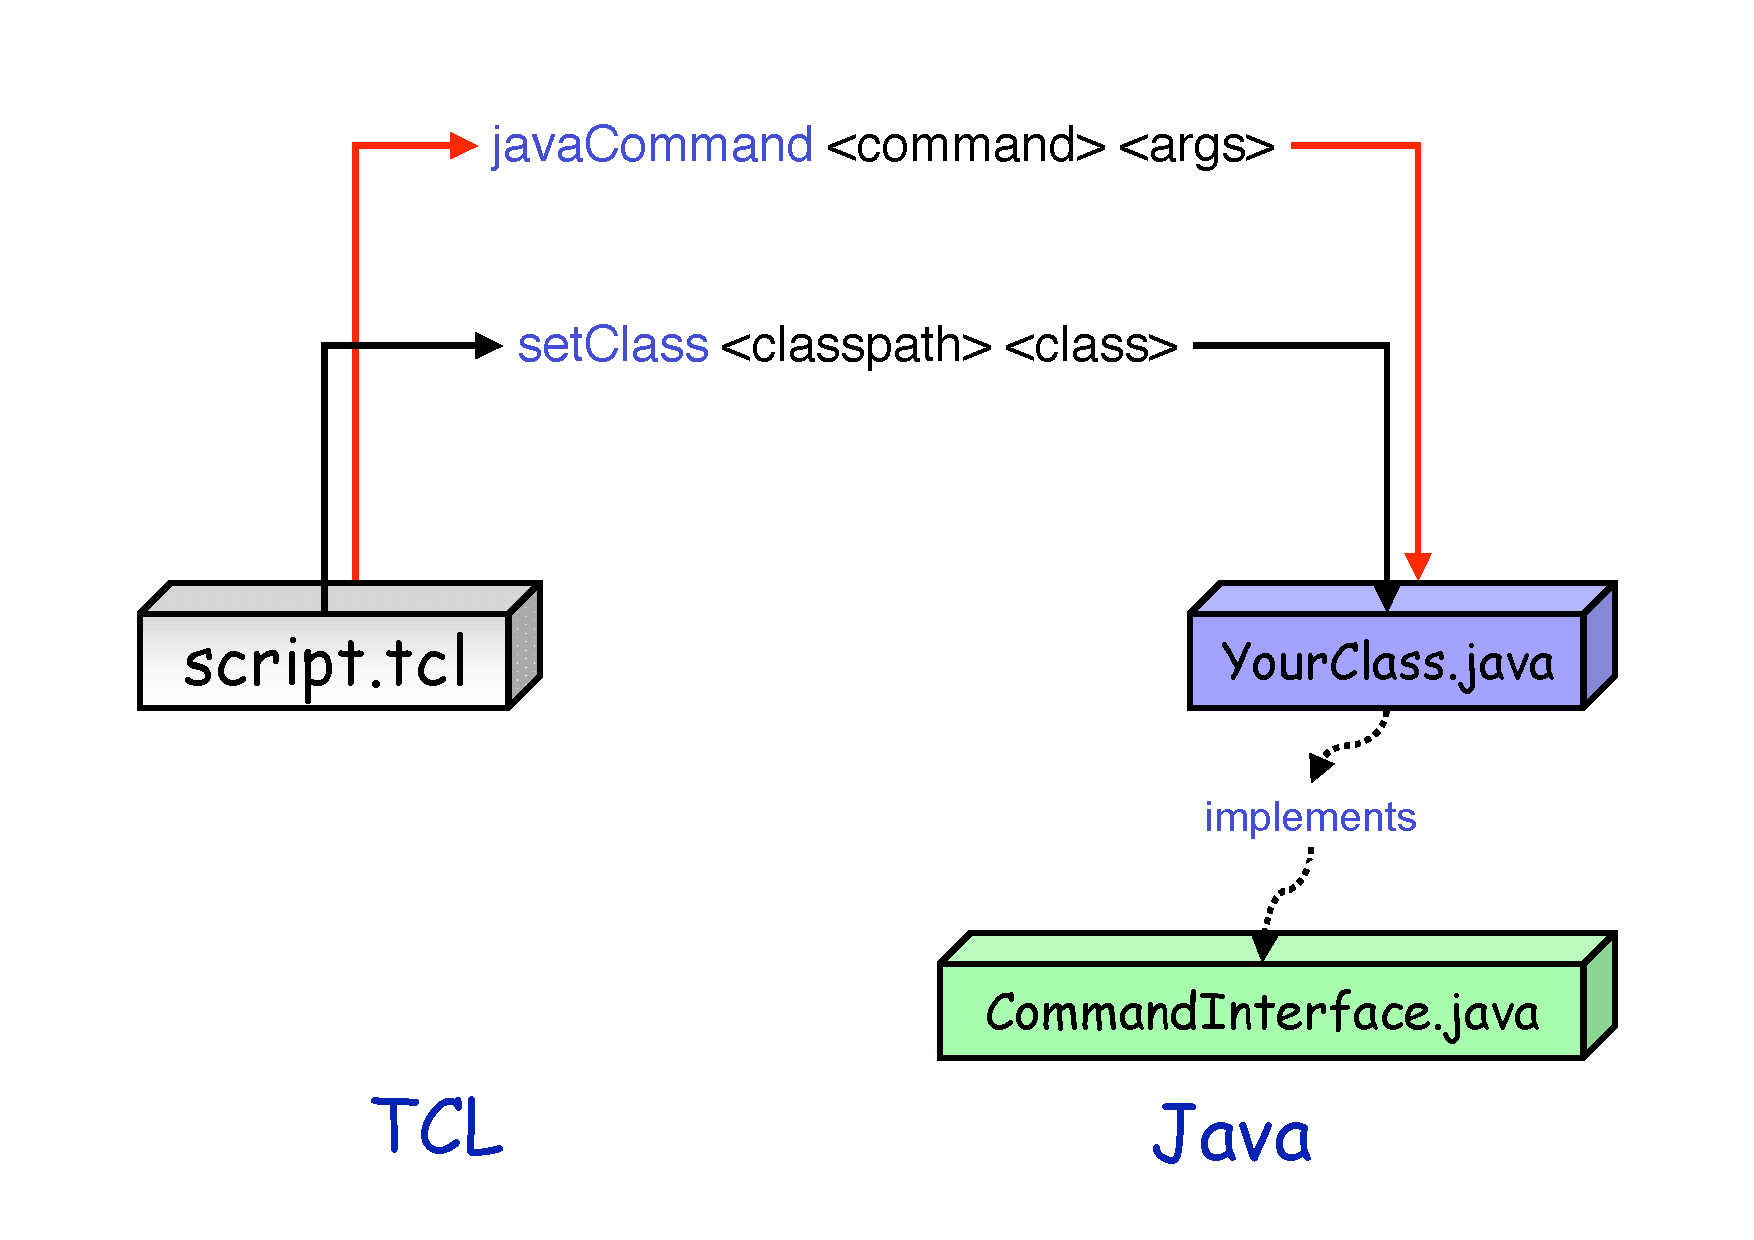
\includegraphics[scale=0.4]{images/agentuserOverview}
\caption{The user's view of the interaction between the NS2 agent/script and
the Java class associated with that NS2 node.} 
\label{jni:fig:javaTCLJava}
\end{figure}

This interaction is shown in Figure \ref{jni:fig:javaTCLJava}, which shows 
some  \emph{JavaAgent} commans for specifying and attaching a Java
object and for sending it commands.  These are the minimum commands 
needed in order to use your Java object.  Each Ns2 node creates a 
Java object of its own choice by using the TCL command:

\footnotesize
\begin{verbatim}
setClass <classpath> <class>
\end{verbatim}
\normalsize

\noindent which allows the Java classpath to be set along with the name of the Java class to be instantiated for this NS2 node. Once the Java object has been created,
commands can be sent by using the TCL command:

\footnotesize
\begin{verbatim}
javaCommand <command> <args>
\end{verbatim}
\normalsize

\noindent which would invoke the java command with the associated 
arguments. There are also other commands implemented that allow you to
specify the delimiter to make it easier to chunk your arguments in a
flexible way and for creating a trigger mechanism.  The following 2
sections illustrate these commands through the use of example
TCL and Java codes and the next chapter illustrates how you
can extend the Java functionality to use PAI in order to send
data between your Java objects through the NS2 subsystem.


\section{Creating and Attaching a Java Agent }
\label{jni:basic}

This is a \emph{Hello World} example that demonstrates how
to specify the Java classpath and choose a Java class to instantiate
and attach to your C++ agent. It then implements a simple \emph{hello}
function which is invoke on the Java object. 

\subsection{The TCL Side}
\label{jni:tclside}

The following is the TCL script part of the implementation, which creates two 
\emph{JavaAgent} NS2 nodes that each create a \emph{SimpleCommand} 
Java object and then invoke a 'hello' command on that object. This
example can be found in examples/pai/javaAgent/startJava.tcl.)

\footnotesize
\begin{verbatim}

puts "Starting..."   

# Create a simulator instance
set ns_ [new Simulator ]

# Create two nodes
set n1 [$ns_ node]
set n2 [$ns_ node]

# Put a link between them
$ns_ duplex-link $n1 $n2 64kb 100ms DropTail
$ns_ queue-limit $n1 $n2 100
$ns_ duplex-link-op $n1 $n2 queuePos 0.5
$ns_ duplex-link-op $n1 $n2 orient right

puts "Creating JavaAgent NS2 agents and attach them to the nodes..."   
set p1 [new Agent/JavaAgent]
$ns_ attach-agent $n1 $p1

set p2 [new Agent/JavaAgent]
$ns_ attach-agent $n2 $p2

puts "CREATED OK          ....... ..." 
    
# Initialize each broker telling it what its NS2 address is

puts "In script: Initializing  ..." 
	
$ns_ at 0.0 "$p1 initAgent"
$ns_ at 0.0 "$p2 initAgent"

puts "Setting Java Object to use by each agent ..." 

$ns_ at 0.0 "$p1 setClass 
/Users/scmijt/Apps/nrl/p2ps-ns2/classes pai.examples.ns2.SimpleCommand"

$ns_ at 0.0 "$p2 setClass 
/Users/scmijt/Apps/nrl/p2ps-ns2/classes pai.examples.ns2.SimpleCommand"

# send a message to each agent and tell it to print it to the screen
# This is a "HelloWorld" program for JavaAgents

$ns_ at 0.0 "$p1 javaCommand hello AStringFromP1" 
$ns_ at 0.0 "$p2 javaCommand hello AStringFromP2" 

$ns_ at 10.0 "finish $ns_"

proc finish {ns_} {
$ns_ halt
delete $ns_
}

$ns_ run
\end{verbatim}
\normalsize

The Java agent parts can be seen in this example.  The \emph{setClass}
function sets the classpath to the \emph{p2ps-ns2} installations classes 
directory.  Here, the actual java class that this node will be using is 
specified as \emph{pai.examples.ns2.SimpleCommand}.  Note 
here that you can load  in classes that are contained in any 
java package that you wish as long as you follow the Java 
conventions for locating the compiled versions of these classes.

Once the Java classes have been located, you can then execute various 
commands by using the \emph{javaCommand} instruction.  Here we
ask the Java class to execute a \emph{hello} command and pass
a string as an argument, identifying the node that is sending the message 
i.e. \emph{AStringFromP1}.  This simple example demonstrates that
two Java objects have been created, one for each node and each Java
object has been correctly associated or bound to the particular NS2
node.

\subsection{The Java Side}
\label{jni:javaside}

On the java side of things each object you want to talk to must implement a 
standard interface called "CommandInterface" which enforces that every Java
object implementing this interface implements this command method:

\footnotesize
\begin{verbatim}
package pai.broker;

public interface CommandInterface {

    public String command(String command, String value);
}
\end{verbatim}
\normalsize

Every class that you wish to be used from an NS2 agent must implement
this Java interface so that it can understand the instructions that are sent
to it. Below, an example Java class is given to illustrate the code involved 
in this process (the actual Java code for this and all other examples 
\sloppypar can be found in the \emph{src/jpai/pai/examples/ns2} directory):

\footnotesize
\begin{verbatim}

package pai.examples.ns2;

import pai.broker.CommandInterface;

public class SimpleCommand implements CommandInterface {

    static int count=0;

    int myID;

    public SimpleCommand() {
        ++count;
        myID=count;
    }

    public String command(String command, String args[]) {

        if (command.equals("hello"))
            System.out.println("SimpleCommand(" + myID + ") 
            					called with Val: " + args[0]);

        return "All called ok from node " + myID;
    }
}

\end{verbatim}
\normalsize

As you can see, this is extremely simple, the C++ and Java JVM class take care of all
the complexity. In the command method, you can implement any behaviour you
want. You can also return a \emph{String} to your C++ 
program as indicited. This could allow you, for example, to discover other 
NS2 nodes using P2PS and then return their
address to your C++ agent and keep the control at this point (helpful for 
non-java programmers!).


\section{Changing the Command Delimiter }
\label{jni:delimiter}

This example demonstrates how you would change the delimiter used
to separate command arguments sent to your Java application.   
The default is to use a white space (as in NS2) to automatically 
parse the arguments and send them as a sequence of arguments
to your agent or Java object.  Within the Java NS2 implementation
however, this choice is left up to the programmer.  Therefore,
you could specify for example a '-' symbol as a delimeter and
a sequence such as this

\begin{verbatim}
8 - cherry apple oranges - to eat
\end{verbatim}

\noindent would be parsed and sent to you program as 3 strings:

\begin{verbatim}
8
cherry apple oranges
to eat
\end{verbatim}

This allows more flexibility in the way you send instructions to your Java
code because it does not limit the input to contiguous strings. The example
given below demonstrates how this is achieved from the TCL and Java 
sides.

\subsection{The TCL Side}
\label{jni:tclside}

The following is the TCL script part of the implementation, which creates two 
\emph{JavaAgent} NS2 nodes that each create a \emph{ChangeDelimiter} 
Java object and then change the delimiter of one of the nodes in order
to split up the input with respect to a '-' symbol.   Note that setting
delimiters is a global process and therefore can be set through 
any node and will be applied to all nodes. This
example can be found in examples/pai/javaAgent/changeDelimiter.tcl)

\footnotesize
\begin{verbatim}
puts "Starting..."   

# Create simulator instance
set ns_ [new Simulator]

# Create two nodes
set n1 [$ns_ node]
set n2 [$ns_ node]

# Put a link between them
$ns_ duplex-link $n1 $n2 64kb 100ms DropTail
$ns_ queue-limit $n1 $n2 100
$ns_ duplex-link-op $n1 $n2 queuePos 0.5
$ns_ duplex-link-op $n1 $n2 orient right
   
puts "Creating JavaAgent NS2 agents and attach them to the nodes..."   
set p1 [new Agent/JavaAgent]
$ns_ attach-agent $n1 $p1

set p2 [new Agent/JavaAgent]
$ns_ attach-agent $n2 $p2
    
puts "In script: Initializing  ..." 
	
$ns_ at 0.0 "$p1 initAgent"
$ns_ at 0.0 "$p2 initAgent"

puts "Setting Java Object to use by each agent ..." 

$ns_ at 0.0 "$p1 setClass 
/Users/scmijt/Apps/nrl/p2ps-ns2/classes pai.examples.ns2.ChangeDelimiter"

$ns_ at 0.0 "$p2 setClass 
/Users/scmijt/Apps/nrl/p2ps-ns2/classes pai.examples.ns2.ChangeDelimiter"

# Delimiters are global and can be set through any node

$ns_ at 0.0 "$p1 javaCommand setDelimiter -" 

$ns_ at 0.0 "$p2 javaCommand hello A-String-From-P2" 

$ns_ at 10.0 "finish $ns_"

proc finish {ns_} {
$ns_ halt
delete $ns_
}

$ns_ run
\end{verbatim}
\normalsize

The Java classes are located and instantiate as previous. Now, we can
use the \emph{javaCommand setDelimiter} instruction to change
the delimiter.  We set this to '-' and then send a single contiguous string
to node p2 (A-String-From-P2) by using the 'hello' command.  Now
instead of passing this as a single string (as you would get in the NS2 
C++ binding), you would get 4 separate string send to your program,
which can be accessed individually, for example, as:

\begin{verbatim}
A
String
From
P2
\end{verbatim}

\subsection{The Java Side}
\label{jni:javaside}

On the java side \emph{ChangeDelimiter.java} implements the
"CommandInterface" to identify that it can process commands:

\footnotesize
\begin{verbatim}
package pai.examples.ns2;

import pai.broker.CommandInterface;

public class ChangeDelimiter implements CommandInterface {

    static int count=0;

    int myID;

    public ChangeDelimiter() {
        ++count;
        myID=count;
    }

    public String command(String command, String args[]) {

        if (command.equals("hello")) {
            System.out.println("Command has "
                    + args.length + " arguments");
            for (int i=0; i<args.length; ++i) {
                System.out.println("Arg[" + i + "] = " + args[i]);
            }
        }

        return "All called ok from node " + myID;
    }
}

\end{verbatim}
\normalsize

Here, the 'hello' command simply processes through the arguments and
prints each to the screen on a separate line. Therefore, running the script 
will produce the following output:

\footnotesize
\begin{verbatim}

In script: Initializing  ...
Setting Java Object to use by each agent ...
Classpath is -Djava.class.path=/Users/scmijt/Apps/nrl/p2ps-ns2/classes
command has 4 arguments
Arg[0] = A
Arg[1] = String
Arg[2] = From
Arg[3] = P2

\end{verbatim}
\normalsize

\section{Conclusion}

Then, two different examples were provided that illustrate how one would
attach a Java object to an NS2 node and how one can execute Java
commands on that object.  Lastly, an example was given that demonstrates
how you can change the delimiter used to parse the list of arguments you
can send to your Java object.  This employs a flexible mechanism that 
can use any string as a delimiter to send lists or sentences to your
Java object without having to parse further. 


